% -*- coding:utf-8 -*-
\documentclass{standalone}
\usepackage{fontspec}
\setmainfont{Times New Roman}
\usepackage[UTF8]{ctex}
\usepackage{tikz}
\usepackage{amsmath}
\usetikzlibrary{matrix,calc,shapes,backgrounds,patterns,positioning,decorations.pathreplacing}
\begin{document}
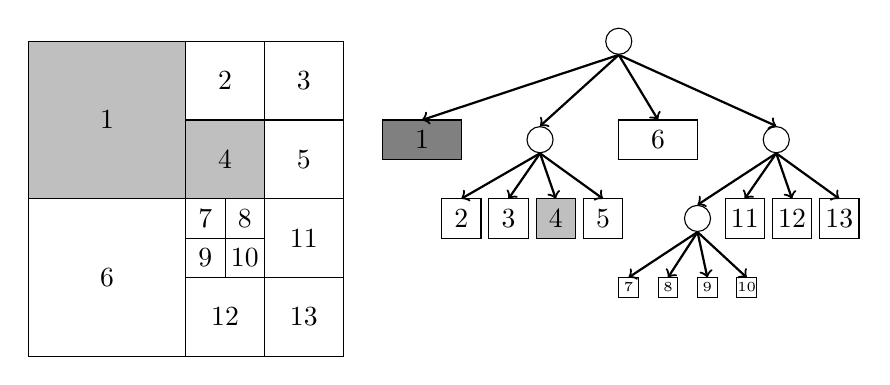
\begin{tikzpicture}
[connection/.style={
	circle,
        draw,
        fill=white,
        radius=1mm,
        minimum size=1mm,
    },]
% draw the left part
\draw (0,0) rectangle (2,2) node at (1,1){$6$};
\draw[fill=gray!50] (0,2) rectangle (2,4) node at (1,3){$1$};
\draw (2,0) rectangle (3,1) node at (2.5,0.5) {$12$};
\draw (3,0) rectangle (4,1) node at (3.5, 0.5) {$13$};
\draw (3,1) rectangle (4,2) node at (3.5, 1.5){$11$};
\draw (2,1) rectangle (2.5,1.5) node at (2.25, 1.25){$9$};
\draw (2.5,1.5) rectangle (3,2) node at (2.75, 1.75){$8$};
\draw (2,1.5) rectangle (2.5,2) node at (2.25, 1.75){$7$};
\draw (2.5,1) rectangle (3, 1.5) node at (2.75, 1.25){$10$};
\draw[fill=gray!50] (2,2) rectangle (3,3) node at (2.5,2.5){$4$};
\draw (3,3) rectangle (4,4) node at (3.5,3.5){$3$};
\draw (2,3) rectangle (3,4) node at (2.5, 3.5){$2$};
\draw (3,2) rectangle (4,3) node at (3.5, 2.5){$5$};

\node[connection] (top) at (7.5,4){};
\draw[fill=gray!=50] (4.5,3) rectangle (5.5,2.5) node at (5, 2.75) {$1$};
\node[connection] (middle1) at (6.5, 2.75){};
\draw (7.5,3) rectangle (8.5, 2.5) node at (8,2.75){$6$};
\node[connection] (middle2) at (9.5, 2.75){};
\draw (5.25,2) rectangle (5.75, 1.5) node at (5.5, 1.75){$2$};
\draw (5.85,2) rectangle (6.35, 1.5) node at (6.1, 1.75){$3$};
\draw[fill=gray!50] (6.45,2) rectangle (6.95, 1.5) node at (6.7, 1.75){$4$};
\draw (7.05,2) rectangle (7.55, 1.5) node at (7.3, 1.75){$5$};

%\draw (5.25+3,2) rectangle (5.75+3, 1.5) node at (5.5+3, 1.75){2};
\node[connection] (latter1) at (8.5, 1.75){};
\draw (8.85,2) rectangle (9.35, 1.5) node at (6.1+3, 1.75){$11$};
\draw[] (9.45,2) rectangle (9.95, 1.5) node at (6.7+3, 1.75){$12$};
\draw (10.05,2) rectangle (10.55, 1.5) node at (7.3+3, 1.75){$13$};

% draw 
\draw[font=\tiny]  (7.5,1) rectangle (7.75,0.75) node at (7.625,0.875){$7$};
\draw[font=\tiny]  (7.8+0.2,1) rectangle (8.05+0.2,0.75) node at (7.925+0.2,0.875){$8$};
\draw[font=\tiny]  (8.1+0.4,1) rectangle (8.35+0.4,0.75) node at (8.225+0.4,0.875){$9$};
\draw[font=\tiny] (8.4+0.6,1) rectangle (8.65+0.6,0.75) node at (8.525+0.6,0.875){$10$};

%draw lines
\draw[thick, ->] (top.south) -- (5,3);
\draw[thick, ->] (top.south) -- (middle1.north);
\draw[thick, ->] (top.south) -- (8,3);
\draw[thick, ->] (top.south) -- (middle2.north);
\draw[thick, ->] (middle1.south) -- (5.5,2);
\draw[thick, ->] (middle1.south) -- (6.1,2);
\draw[thick, ->] (middle1.south) -- (6.7,2);
\draw[thick, ->] (middle1.south) -- (7.3,2);
\draw[thick, ->] (middle2.south) -- (latter1.north);
\draw[thick,->] (middle2.south) -- (9.1, 2);
\draw[thick,->] (middle2.south) -- (9.7, 2);
\draw[thick,->] (middle2.south) -- (10.3, 2);
\draw[thick, ->] (latter1.south) -- (7.625,1);
\draw[thick, ->] (latter1.south) -- (7.925+0.2,1);
\draw[thick, ->] (latter1.south) -- (8.225+0.4,1);
\draw[thick, ->] (latter1.south) -- (8.525+0.6,1);
\end{tikzpicture}
\end{document}